%\documentclass[fleqn,14pt,a4paper,twoside]{extarticle}
\documentclass[a4paper, 11pt]{extarticle}
%\usepackage[tmargin=4cm,bmargin=4cm,lmargin=2cm,rmargin=2cm,asymmetric,headheight=50pt,bindingoffset=1cm]{geometry}
\usepackage[tmargin=1.5cm,bmargin=1.5cm,lmargin=2cm,rmargin=1.5cm,headheight=50pt]{geometry}
\usepackage{comment} % enables the use of multi-line comments (\ifx \fi) 
\usepackage{lipsum} %This package just generates Lorem Ipsum filler text. 
\usepackage{fullpage} % changes the margin
%\usepackage[a4paper, total={7in, 10in}]{geometry}
\usepackage[fleqn]{amsmath}
\usepackage{amssymb,amsthm}  % assumes amsmath package installed
\newtheorem{theorem}{Theorem}
\newtheorem{corollary}{Corollary}
\usepackage{graphicx}
\usepackage{tikz}
\usetikzlibrary{arrows}
\usepackage{verbatim}
\usepackage[numbered]{mcode}
\usepackage{float}
\usepackage{tikz}
    \usetikzlibrary{shapes,arrows}
    \usetikzlibrary{arrows,calc,positioning}

    \tikzset{
        block/.style = {draw, rectangle,
            minimum height=1cm,
            minimum width=1.5cm},
        input/.style = {coordinate,node distance=1cm},
        output/.style = {coordinate,node distance=4cm},
        arrow/.style={draw, -latex,node distance=2cm},
        pinstyle/.style = {pin edge={latex-, black,node distance=2cm}},
        sum/.style = {draw, circle, node distance=1cm},
    }
\usepackage{xcolor}
\usepackage{mdframed}
\usepackage[shortlabels]{enumitem}
%\usepackage{indentfirst}
\usepackage{hyperref}
    
\renewcommand{\thesubsection}{\thesection.\alph{subsection}}

\newenvironment{problem}[2][Problem]
    { \begin{mdframed}[backgroundcolor=gray!20] \textbf{#1 #2} \\}
    {  \end{mdframed}}

% Define solution environment
\newenvironment{solution}
    {\textit{Solution:}}
    {}

\renewcommand{\qed}{\quad\qedsymbol}


\usepackage{fancyhdr}
\usepackage{emptypage}
\fancyhead{}
\fancyfoot{}
\fancyhead[LE,RO]{
\includegraphics [width=.3\textwidth] {logo.png}}
\fancyfoot[LE,RO]{\thepage}
\pagestyle{fancy}
\graphicspath{{../../tex_templates/figures/}}

%%%%%%%%%%%%%%%%%%%%%%%%%%%%%%%%%%%%%%%%%%%%%%%%%%%%%%%%%%%%%%%%%%%%%%%%%%%%%%%%%%%%%%%%%%%%%%%%%%%%%%%%%%%%%%%%%%%%%%%%%%%%%%%%%%%%%%%%
\begin{document}
%Header-Make sure you update this information!!!!
\noindent
%%%%%%%%%%%%%%%%%%%%%%%%%%%%%%%%%%%%%%%%%%%%%%%%%%%%%%%%%%%%%%%%%%%%%%%%%%%%%%%%%%%%%%%%%%%%%%%%%%%%%%%%%%%%%%%%%%%%%%%%%%%%%%%%%%%%%%%%
\large{\textbf{Course: WebDev -- Django Start.}} \hfill  \\ 
\vspace{0.25em}
\textbf{Homework - 1}  \hfill  \\
%Email: veralevel@gethu.edu \hfill ID: 123456789 \\

Theme: Install instruments for work and basic \hfill  \\
Level: beginner\\
Instructor: Mikhail Nakonechnyi \\
Due Date: $15^{th}$ February, 2020 \\
\noindent\rule{7in}{2.8pt}
%%%%%%%%%%%%%%%%%%%%%%%%%%%%%%%%%%%%%%%%%%%%%%%%%%%%%%%%%%%%%%%%%%%%%%%%%%%%%%%%%%%%%%%%%%%%%%%%%%%%%%%%%%%%%%%%%%%%%%%%%%%%%%%%%%%%%%%%
% Problem 1
%%%%%%%%%%%%%%%%%%%%%%%%%%%%%%%%%%%%%%%%%%%%%%%%%%%%%%%%%%%%%%%%%%%%%%%%%%%%%%%%%%%%%%%%%%%%%%%%%%%%%%%%%%%%%%%%%%%%%%%%%%%%%%%%%%%%%%%%
\begin{problem}{1}
Consider the scalar system
\begin{align*}
    \Dot{x} &= -x + u + w
\end{align*}
$w$ is zero-mean process noise with a variance of $Q$. The control has a mean value of $u_0$, an uncertainty of $2$ (one standard deviation), and is uncorrelated with $w$. Rewrite the system equations to obtain an equivalent system with a normalized control that is perfectly known. What is the variance of the new process noise term in the transformed system equation?
\end{problem}
\begin{solution}
The variance of the new process noise, $w_u$ is $\Sigma_{w_{u}} = Q + \sigma^2_u = Q + 4$.
\begin{align*}
    \Dot{x} &= -x + u_0 + \underbrace{w + \Delta u}_{w_{u}}, \quad w_u \sim (0, Q + \sigma^2_u).
\end{align*}
\end{solution} 
\noindent\rule{7in}{2.8pt}

%%%%%%%%%%%%%%%%%%%%%%%%%%%%%%%%%%%%%%%%%%%%%%%%%%%%%%%%%%%%%%%%%%%%%%%%%
% Problem 2
%%%%%%%%%%%%%%%%%%%%%%%%%%%%%%%%%%%%%%%%%%%%%%%%%%%%%%%%%%%%%%%%%%%%%%%%%%%%%%%%%%%%%%%%%%%%%%%%%%%%%%%%%%%%%%%%%%%%%%%%%%%%%%%%%%%%%%%%

\begin{problem}{2}
Consider the system
\begin{align*}
    x_{k+1} &= \phi x_{k} + w_{k}, \\
    y_k &= x_k, 
\end{align*}
where $w_k \sim (0, 1)$, and $\phi = 0.9$ is an unknown constant. Design an extended Kalman filter to estimate $\phi$. Simulate the filter for $100$ time steps with $x_0 = 1, P_0 = I , \hat{x}_{0} = 0$, and $\hat{\phi}_{0} = 0$. Hand in your source code and a plot showing $\hat{\phi}$ as a function of time.
\end{problem}
\begin{solution}
Perform the measurement update of the state estimate and estimation error covariance as follows
\begin{align*}
    K_k &= P^{-}_k H^{\top}_k (H_k P^{-}_k H^{\top}_k + R_k)^{-1} = P^{-}_k H^{\top}_k (H_k P^{-}_k H^{\top}_k)^{-1}, \quad \text{Since }R_k = 0, \\
    \hat{\bar{x}}^{+}_{k} &= \hat{\bar{x}}^{-}_{k} + K_k (y_k - h_k(\hat{\bar{x}}^{-}_{k}, 0)) \\
    &= \hat{\bar{x}}^{-}_{k} + K_k (y_k - \hat{x}^{-}_{k}), \quad \text{Since } \hat{\phi}^{-}_{k} = 0, \\
    P^{+}_k &= (I - K_k H_k) P^{-}_k
\end{align*}
\begin{figure}[H]
    \centering
    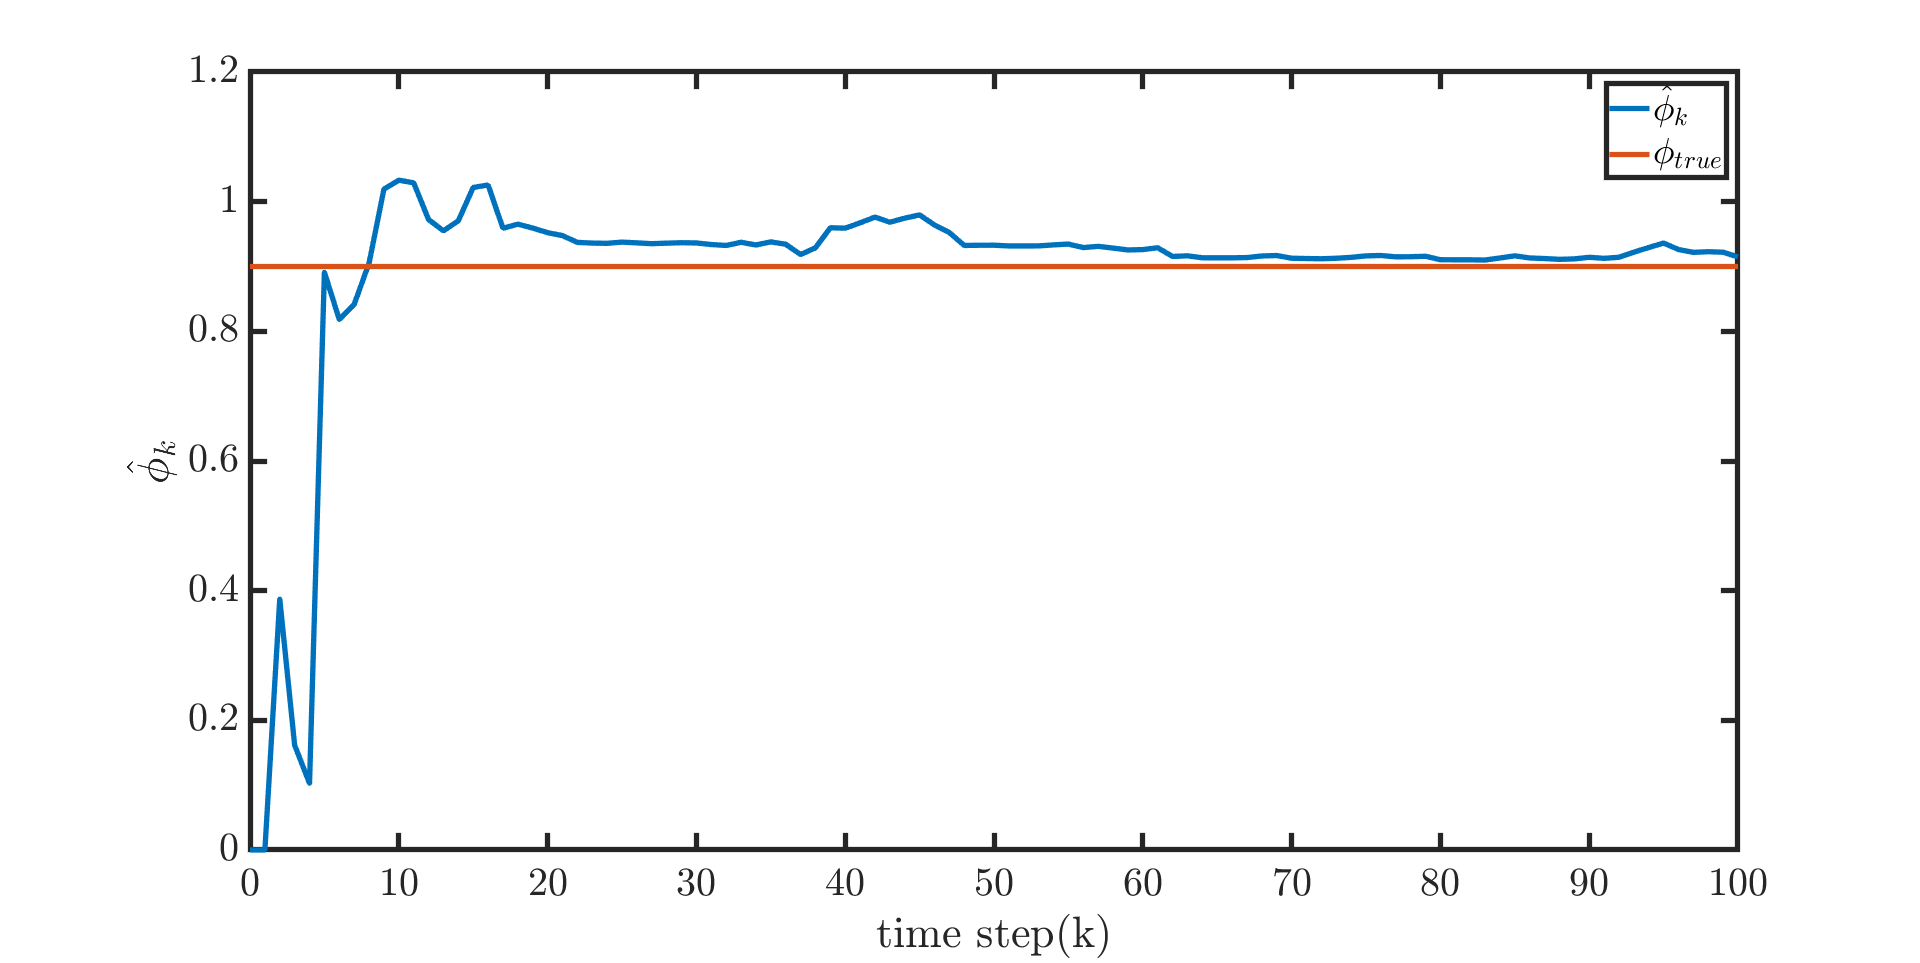
\includegraphics[scale=0.25]{q2.png}
    \caption{Plot showing $\hat{\phi}$ as a function of time.}
    \label{fig_q2l}
\end{figure}
\end{solution} 
\lstinputlisting{HW6Q2.m}
\noindent\rule{7in}{2.8pt}
%%%%%%%%%%%%%%%%%%%%%%%%%%%%%%%%%%%%%%%%%%%%%%%%%%%%%%%%%%%%%%%%%%%%%%%%%
\end{document}
 